To evaluate the optimization result, we test the implementation in a 64 bit Arch Linux machine with Intel CPU of Skylake i7-6600U CPU @ 3GHz. The compiler and arithmetic environment are as following: 

  \begin{itemize}
  \setlength\itemsep{0.5em}
  \item{GCC 6.1.1 compiler}
  \item{64 bit multiplication (mul, mulx): 1 op/cycle}
  \item{64 bit addition/subtraction (add, sub): 4 op/cycle}
  \item{64 bit addition with carry (adc, adcx, adox): 1 op/cycle}
  \item{Carry addition only: peak performance of 2 ops/cycle ~6 Gops/s on 1 core}
  \item{Compile flag: -O3 -mavx2 -mbmi2 -madx}
  \end{itemize}
  \setlength\itemsep{1.5em}
Based on the recommended Elliptic curve parameters from the guidance standard \cite{Brown:2009}, we have chosen 5 predefined curves with various key size : 192, 224, 256, 384, 521 bits.All versions of implementation has been validated by using Google Unit test, by checking the key exchange result. The benchmark is done by calculating the CPU cycles, in order to testify the real performance by eliminating the influence of the machine. In the end we compare our implementation with OpenSSL, the well known open source library to check our implementation effect. The OpenSSL ECDH mechanism is deployed and the library has been imported as a package of GCC.


\begin{figure}[h!]\centering
  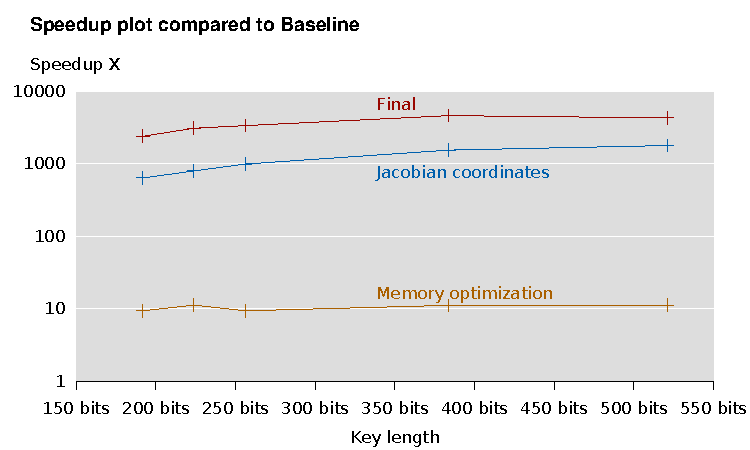
\includegraphics[scale=0.7]{speedup}
  \caption{Speedup plot compared to Baseline \label{speedup}}
\end{figure}
\begin{figure}[h!]\centering
  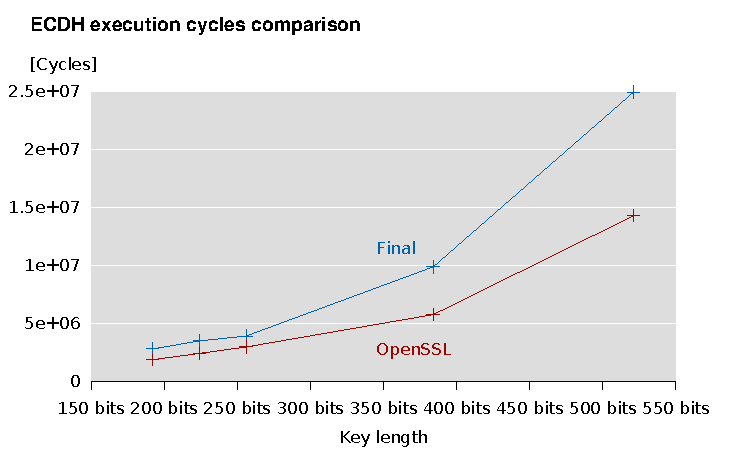
\includegraphics[scale=0.7]{ecdh}
  \caption{ECDH execution cycles comparison\label{ecdh}}
\end{figure}
\begin{figure}[h!]\centering
  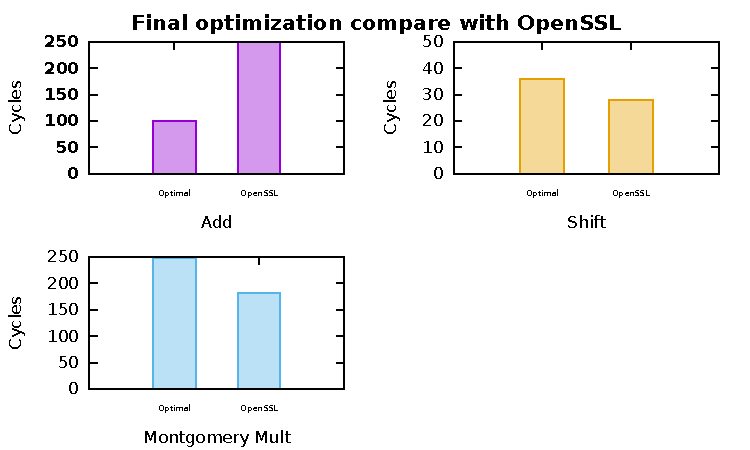
\includegraphics[scale=0.7]{openssl}
  \caption{Final optimization compared with OpenSSL\label{openssl}}
\end{figure}

In the speedup comparison(Fig.~\ref{speedup}) three crucial numbers are shown. It can be clearly seen that the Final implementation can execute the key exchange process 5000 times faster than the baseline in almost all the key lengths. In all three cases the speedup increases as the key size grows. It can be explained that the program is not fully functioning when the key size is relatively small, considering that the big integer operations(64 bits base) will take full operations even with smaller input size. The first milestone of memory optimization gives us about 10 times speedup, whereas Jacobian coordinates can run 1000 times faster. The speedup result is satisfactory and reasonable as the baseline implementation contains costly and expensive memory allocations. 



Next we run the same operation with OpenSSL library and compare their computation cycles with us. It is no surprise that with the increasing of the key length the required cycles also increase rapidly(Fig.~\ref{ecdh}). Our required cycles remain the save level with OpenSSL with key length smaller than 256 bits, yet fall behind OpenSSL with larger key length. 



Individual operations of integers are the main component of our algorithm. To see how good is our implementation we chose integer addition, shift and Montgomery multiplication to compare with OpenSSL(Fig.~\ref{openssl}).This comparison is done with fixed key length of 192 bits. In the comparison of integer addition, our final implementation uses less cycles than OpenSSL big integer addition thus being faster than OpenSSL. Yet in both shift and Montgomery multiplication our implementation is more expensive and slower than OpenSSL. 

\begin{figure}[h!]\centering
  \includegraphics[scale=0.7]{perfplot1}
  \caption{Performance plot of baseline and memory optimization\label{perfplot1}}
\end{figure}
\begin{figure}[h!]\centering
  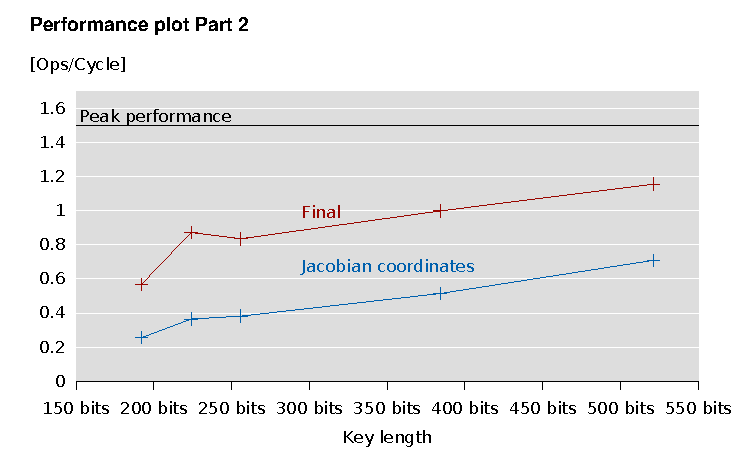
\includegraphics[scale=0.7]{perfplot2}
  \caption{Performance plot of Final optimization and Jacobian coordinates\label{perfplot2}}
\end{figure}

Performance plots(Fig.~\ref{perfplot1} and Fig.~\ref{perfplot2}) are consisted with the division of operation counts and cycles. It reflects if the implementation can reach up the machines' computation ability. Normal operations counts would stay constant as the optimization goes on. Yet in our case since the integer operations does not only include the normal integer operations, but also include the index counts. Thus we have to compromise by using code generated operation counts. In the following performance plot the operation counts changes, but it does reflect the computational efficiency of the code in certain level. In Fig.~\ref{perfplot1} the first comparison is done by showing the effect of memory optimization. It is clear that with huge amount of memory allocation, the baseline performance is really limited. In Fig.~\ref{perfplot2} we begin to see the real performance boost that comes from later optimization. The peak performance here is calculated by considering the ratio of additions and multiplications. With 1 add and 1 mult per cycle and two times add versus one mult, we can draw the line of peak performance at 1.5 ops/cycle. As we can see the final optimization are close to the peak performance with large key size, proving the optimization work successful.


\begin{figure}[h!]\centering
  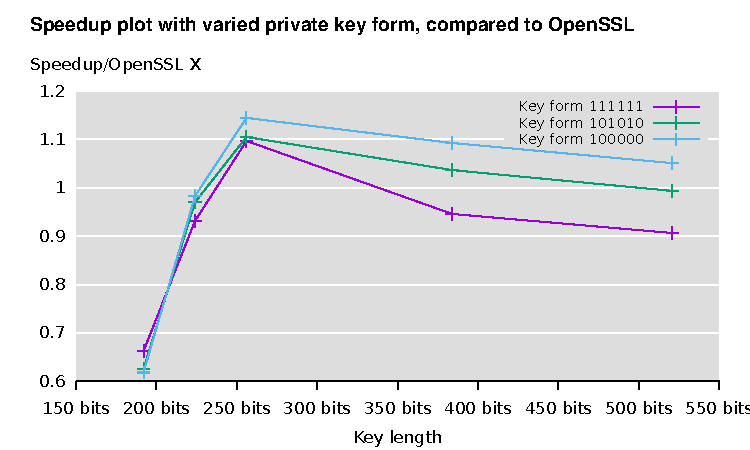
\includegraphics[scale=0.7]{keysize}
  \caption{Speedup plot with varied private key form, compared to OpenSSL\label{keysize}}
\end{figure}
Fig.~\ref{perfplot1} gives us another perspective of how different key form would influence the speedup. In the simplified private key form that consist of only zeros and ones, our speed of processing EDCH come closely to OpenSSL. The key form that consist only ones has the worst performance since it requires redundant integer operations that are unavoidable. 